\documentclass[a4paper,oneside,12pt]{report}
% Package yang diperlukan
\usepackage[table]{xcolor} % Untuk menggunakan warna
\usepackage{graphicx}      % Untuk memasukkan gambar
\usepackage{titling}       % Untuk kustomisasi halaman judul
\usepackage{geometry}      % Untuk mengatur margin halaman
\usepackage{listings}      % Untuk menampilkan blok kode
\usepackage{float}         % Untuk kontrol penempatan float (seperti gambar)
\usepackage{hyperref}      % Untuk membuat hyperlink (URL, referensi)
\usepackage{indentfirst}   % Untuk memberi indentasi pada paragraf pertama setiap seksi
\usepackage{url}           % Untuk format URL
\usepackage{fancyhdr}      % Untuk kustomisasi header dan footer
\usepackage{tocloft}       % Untuk kustomisasi Daftar Isi
\usepackage{bookmark}      % Untuk manajemen bookmark PDF yang lebih baik
\usepackage{amsmath}       % Untuk notasi matematika
\usepackage[most]{tcolorbox} % Untuk box output terminal

% Paket untuk tabel agar sesuai format referensi
\usepackage{array}
\usepackage{booktabs}
\usepackage{tabularx}
\usepackage{multirow}
\usepackage{colortbl}

% Macro untuk header tabel
\newcommand{\thead}[1]{\textcolor{white}{\textbf{#1}}}

%======================================================================
% PENGATURAN GEOMETRI HALAMAN
%======================================================================
\geometry{left=3cm, right=2.5cm, top=2cm, bottom=2.5cm}
\sloppy

%======================================================================
% PENGATURAN WARNA UNTUK BLOK KODE
%======================================================================
\definecolor{codegreen}{rgb}{0,0.6,0}
\definecolor{codegray}{rgb}{0.5,0.5,0.5}
\definecolor{codepurple}{rgb}{0.58,0,0.82}
\definecolor{backcolour}{rgb}{0.95,0.95,0.92}
\definecolor{darkblue}{rgb}{0,0,0.6}
\definecolor{outputbg}{RGB}{241,245,249}
\definecolor{outputborder}{RGB}{203,213,225}

%======================================================================
% PENGATURAN BLOK KODE (LISTINGS)
%======================================================================
\lstdefinestyle{commonstyle}{
    backgroundcolor=\color{backcolour},
    breakatwhitespace=false,
    breaklines=true,
    captionpos=b,
    keepspaces=true,
    numbers=left,
    numbersep=5pt,
    showspaces=false,
    showstringspaces=false,
    showtabs=false,
    tabsize=2,
    frame=single,
    basicstyle=\ttfamily\footnotesize,
    numberstyle=\tiny\color{codegray},
    columns=flexible,
    postbreak=\mbox{\textcolor{red}{$\hookrightarrow$}\space},
    breakindent=0pt,
    breakautoindent=false
}

\lstdefinestyle{pythonstyle}{
    style=commonstyle,
    language=Python,
    commentstyle=\color{codegreen},
    keywordstyle=\color{darkblue},
    stringstyle=\color{codepurple},
    emph={import,from,class,def,for,while,if,else,elif,try,except,finally,as,lambda,return},
    emphstyle=\color{darkblue}
}

% ── Box Format Output / Terminal Box (Verbatim via tcblisting) ───────────
\newtcblisting{outputbox}{
    enhanced,
    colback=outputbg,
    colframe=outputborder,
    boxrule=0.6pt,
    arc=1.2mm,
    left=3mm,
    right=3mm,
    top=1.2mm,
    bottom=1.2mm,
    listing only,
    listing options={
        basicstyle=\ttfamily\footnotesize,
        breaklines=true,
        numbers=none,
        showstringspaces=false
    }
}

\newcommand{\screenshotimage}[3]{%
    \begin{figure}[H]
        \centering
        \includegraphics[width=0.85\textwidth]{#1}
        \caption{#2}
        \label{fig:#3}
    \end{figure}
}

%======================================================================
% PENGATURAN LAIN-LAIN
%======================================================================
\renewcommand{\figurename}{Gambar}
\renewcommand{\thefigure}{\arabic{figure}}
\renewcommand{\tablename}{Tabel}

\hypersetup{
    colorlinks=true,
    linkcolor=black,
    filecolor=black,
    urlcolor=black,
    citecolor=black,
    pdftitle={Laporan Praktikum Penambangan Data - Pertemuan III},
    pdfpagemode=FullScreen,
    breaklinks=true
}

\pagestyle{fancy}
\fancyhf{}
\fancyfoot[C]{\thepage}
\renewcommand{\headrulewidth}{0pt}

\fancypagestyle{plain}{
    \fancyhf{}
    \fancyfoot[C]{\thepage}
    \renewcommand{\headrulewidth}{0pt}
}

%======================================================================
% PENGATURAN STRUKTUR BAB DAN DAFTAR ISI
%======================================================================
\renewcommand{\contentsname}{Daftar Isi}
\renewcommand{\bibname}{Daftar Pustaka}

\renewcommand{\thechapter}{}
\renewcommand{\chaptername}{}

\renewcommand{\thesection}{\arabic{chapter}.\arabic{section}}
\renewcommand{\thesubsection}{\thesection.\arabic{subsection}}

\setcounter{secnumdepth}{3}
\setcounter{tocdepth}{3}

\renewcommand{\cftchapdotsep}{\cftdotsep}
\renewcommand{\cftchapleader}{\cftdotfill{\cftchapdotsep}}
\setlength{\cftchapindent}{0em}
\setlength{\cftsecindent}{2em}
\setlength{\cftsubsecindent}{4em}
\setlength{\cftchapnumwidth}{0em}
\setlength{\cftsecnumwidth}{2.5em}
\setlength{\cftsubsecnumwidth}{3.2em}
\renewcommand{\cftchappresnum}{}
\renewcommand{\cftchapaftersnum}{}

%======================================================================
% AWAL DOKUMEN
%======================================================================
\begin{document}

\newgeometry{left=3cm, right=2.5cm, top=2.5cm, bottom=3cm}
\begin{titlingpage}
\begin{center}
\vspace*{0.5cm}
{\large \textbf{\MakeUppercase{Laporan Praktikum}}} \\[0.4cm]
{\large \textbf{\MakeUppercase{Praktikum Penambangan Data}}} \\[0.4cm]
{\large \textbf{\MakeUppercase{Pertemuan III}}} \\[0.4cm]
{\large \textbf{\MakeUppercase{Classification}}} \\[1.5cm]


\includegraphics[height=7cm]{lambang ugm.png} \\[1cm]

{\normalsize \textbf{Disusun oleh:}} \\[0.4cm]
\begin{tabular}{@{}l l @{}}
  \textbf{Nama}           & : Januarsyah Akbar \\
  \textbf{NIM}            & : 24/535846/SV/24314 \\
  \textbf{Kelas}          & : B2 \\
  \textbf{Dosen Pengampu} & : Dr. Ganjar Alfian, S.T., M.Eng. \\
                          & \phantom{:} Dr. Imam Fahrurrozi, S.T., M.Cs.
\end{tabular} \\[1.2cm]

{\normalsize \textbf{PROGRAM STUDI D-IV}} \\[0.2cm]
{\normalsize \textbf{TEKNOLOGI REKAYASA PERANGKAT LUNAK}} \\[0.2cm]
{\normalsize \textbf{DEPARTEMEN TEKNIK ELEKTRO DAN INFORMATIKA}} \\[0.2cm]
{\normalsize \textbf{SEKOLAH VOKASI}} \\[0.2cm]
{\normalsize \textbf{UNIVERSITAS GADJAH MADA}} \\[0.2cm]
{\normalsize \textbf{YOGYAKARTA}} \\[0.2cm]
{\normalsize \textbf{2026}} \\[1.2cm]
\end{center}
\end{titlingpage}
\restoregeometry

\thispagestyle{empty}
\clearpage
\stepcounter{page}
\thispagestyle{empty}

% --- Daftar Isi ---
\addcontentsline{toc}{chapter}{Daftar Isi}
\tableofcontents
\clearpage

\pagenumbering{arabic}
\setcounter{page}{3}

%======================================================================
% BAB I: TUJUAN PRAKTIKUM
%======================================================================
\chapter[Tujuan Praktikum]{Tujuan Praktikum}
Tujuan pelaksanaan praktikum pada Pertemuan III adalah sebagai berikut:
\begin{enumerate}
    \item Mahasiswa mampu memahami konsep dasar beberapa algoritma klasifikasi, seperti Logistic Regression, KNN, Decision Tree, dan Random Forest.
    \item Mahasiswa mengetahui fungsi dan peran metrik evaluasi klasifikasi, seperti accuracy, precision, dan recall dalam menilai performa model.
    \item Mahasiswa dapat menerapkan berbagai algoritma klasifikasi untuk membangun model yang mampu memprediksi kelas dari data baru.
    \item Mahasiswa mampu melakukan evaluasi model dengan menyusun tabel performa berisi accuracy, precision, dan recall dari setiap model.
\end{enumerate}
\clearpage

%======================================================================
% BAB II: DASAR TEORI
%======================================================================
\chapter{Dasar Teori}

\section{Classification}
Klasifikasi merupakan salah satu teknik \textit{supervised learning} yang bertujuan untuk memprediksi label atau kategori dari sebuah sampel berdasarkan fitur yang dimiliki. Model klasifikasi belajar dari data historis berlabel, kemudian menghasilkan fungsi yang mampu menentukan kelas dari data baru yang belum pernah dilihat. Klasifikasi umum digunakan dalam aplikasi seperti deteksi spam, diagnosis medis, dan rekomendasi \cite{ref1,ref4}.

\section{Algoritma Classification}
Beberapa algoritma klasifikasi yang umum digunakan antara lain \cite{ref6}:
\begin{enumerate}
    \item \textbf{Logistic Regression}: Algoritma klasifikasi berbasis regresi linier yang memodelkan probabilitas sampel menggunakan fungsi sigmoid. Output model berada dalam rentang 0-1 yang dikonversi menjadi kelas.
    \item \textbf{K-Nearest Neighbors (KNN)}: Mengklasifikasikan data berdasarkan mayoritas kelas dari \textit{k} tetangga terdekatnya menggunakan perhitungan jarak seperti jarak \textit{Euclidean}.
    \item \textbf{Decision Tree}: Membagi dataset secara rekursif berdasarkan kriteria pemisahan fitur yang memberikan informasi terbaik (seperti \textit{entropy} atau \textit{Gini impurity}).
    \item \textbf{Random Forest}: Algoritma \textit{ensemble} yang menggabungkan banyak \textit{Decision Tree} melalui teknik \textit{bagging} untuk mengurangi varians (\textit{overfitting}) dan menstabilkan prediksi.
    \item \textbf{AdaBoost (Adaptive Boosting)}: Algoritma klasifikasi \textit{ensemble boosting} yang menggabungkan beberapa \textit{weak learners}. Algoritma ini secara sekuensial menyesuaikan bobot untuk berfokus pada data yang salah diprediksi sebelumnya.
\end{enumerate}

\section{Metrik Evaluasi Classification}
Evaluasi performa klasifikasi dilakukan menggunakan komponen \textit{Confusion Matrix} yang memuat \textit{True Positive} (TP), \textit{True Negative} (TN), \textit{False Positive} (FP), dan \textit{False Negative} (FN) \cite{ref4}:
\begin{itemize}
    \item \textbf{Accuracy}: Rasio prediksi benar terhadap total seluruh data yang diprediksi.
    \item \textbf{Precision}: Tingkat ketepatan prediksi kelas positif; seberapa banyak hasil positif dari prediksi yang benar-benar merupakan kelas positif.
    \item \textbf{Recall}: Kemampuan model menemukan seluruh data kelas positif secara benar.
    \item \textbf{F1-Score}: Rata-rata harmonik antara \textit{precision} dan \textit{recall}, digunakan utamanya saat dataset tidak seimbang (\textit{imbalanced data}).
\end{itemize}
\clearpage

%======================================================================
% BAB III: HASIL DAN PEMBAHASAN
%======================================================================
\chapter{Hasil dan Pembahasan}

\section{Langkah Percobaan (Stroke Prediction Dataset)}
Pada bagian pertama, percobaan pemodelan klasifikasi diterapkan pada dataset \textit{Stroke Prediction} untuk mendeteksi risiko stroke.

\begin{enumerate}
    \item \textbf{Load Dataset Stroke} \\
    Dataset dimuat dari repositori dan ditinjau distribusi kategori fitur target \texttt{stroke}.
\begin{lstlisting}[style=pythonstyle, caption=Visualisasi Pie Chart Target Stroke]
data = df['stroke'].value_counts()
plt.pie(data, labels=data.index, autopct='%.2f%%')
plt.show()
\end{lstlisting}
    \screenshotimage{gambar/pie_stroke.png}{Pie Chart Distribusi Target Stroke}{pie_stroke}
    Berdasarkan diagram lingkaran tersebut, kelas negatif (tidak stroke) mendominasi sebesar 95.13\%, sedangkan kelas positif (stroke) hanya 4.87\%. Dataset bersifat sangat \textit{imbalanced}.

    \item \textbf{Visualisasi Distribusi Numerik} \\
    Dilakukan pengecekan distribusi fitur menggunakan histogram.
    \screenshotimage{gambar/hist_stroke.png}{Histogram Variabel Numerik Dataset Stroke}{hist_stroke}

    \item \textbf{Pemodelan dan Evaluasi} \\
    Setelah menangani nilai kosong pada atribut \texttt{bmi}, merubah kategori teks menggunakan \texttt{LabelEncoder}, dan menyelaraskan skala melalui \texttt{StandardScaler}, data dievaluasi dengan beberapa model machine learning (rasio pembagian 70:30).

    Berikut adalah representasi visualisasi \textit{Confusion Matrix} (\textit{heatmap}) untuk masing-masing algoritma, yang menampakkan kecenderungan model terhadap bias kelas mayoritas.

    \begin{figure}[H]
        \centering
        \begin{minipage}{0.45\textwidth}
            \centering
            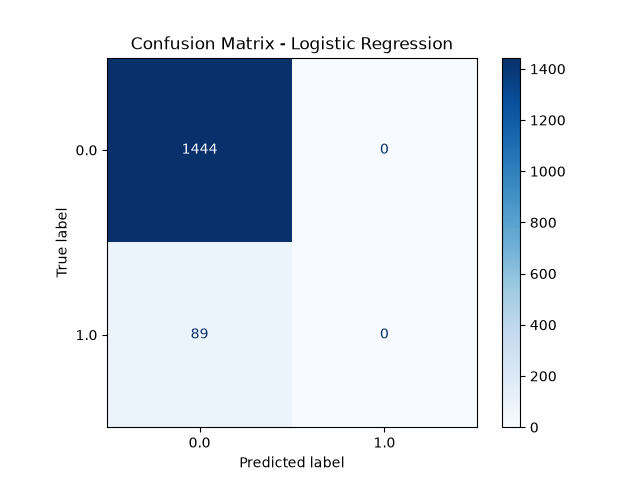
\includegraphics[width=\textwidth]{gambar/cm_lr.png}
            \caption{CM Logistic Regression}
        \end{minipage}\hfill
        \begin{minipage}{0.45\textwidth}
            \centering
            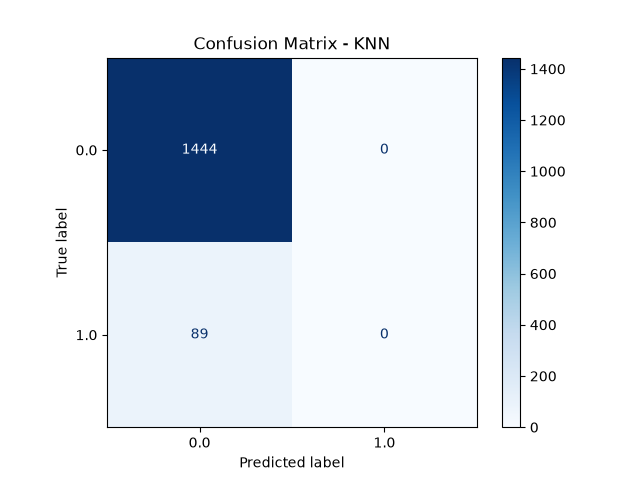
\includegraphics[width=\textwidth]{gambar/cm_knn.png}
            \caption{CM K-Nearest Neighbors}
        \end{minipage}
        
        \vspace{0.5cm}
        \begin{minipage}{0.45\textwidth}
            \centering
            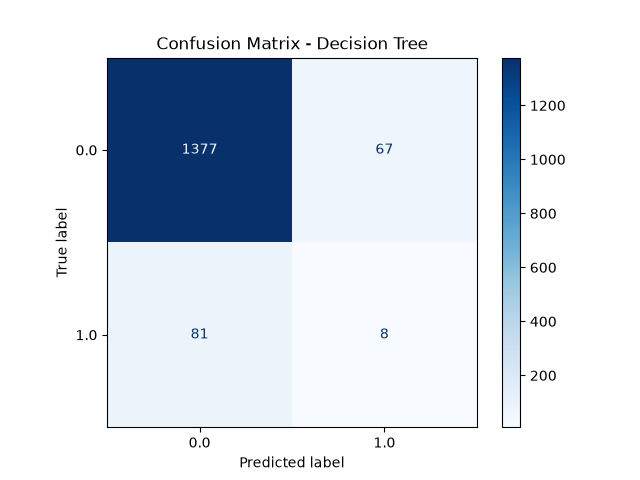
\includegraphics[width=\textwidth]{gambar/cm_dt.png}
            \caption{CM Decision Tree}
        \end{minipage}\hfill
        \begin{minipage}{0.45\textwidth}
            \centering
            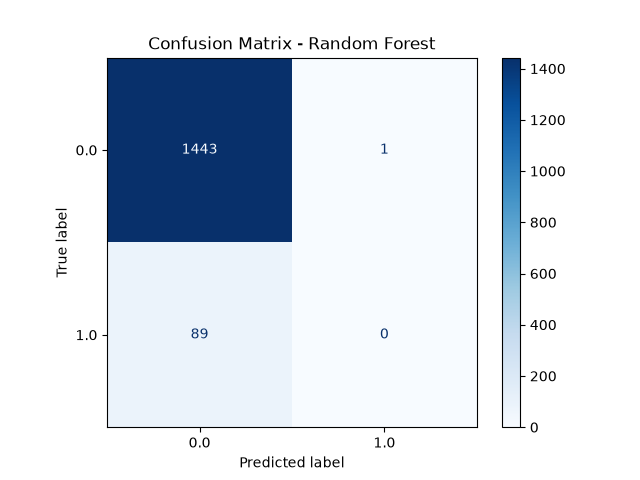
\includegraphics[width=\textwidth]{gambar/cm_rf.png}
            \caption{CM Random Forest}
        \end{minipage}
        
        \vspace{0.5cm}
        \begin{minipage}{0.45\textwidth}
            \centering
            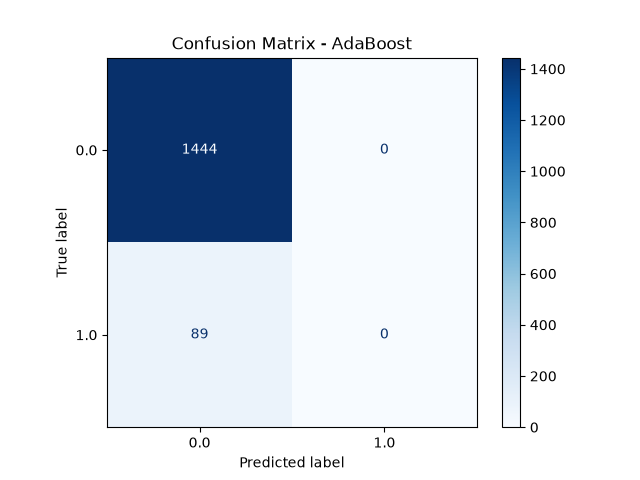
\includegraphics[width=\textwidth]{gambar/cm_ada.png}
            \caption{CM AdaBoost}
        \end{minipage}
    \end{figure}
\end{enumerate}

\section{Tugas dan Analisis (Loan Status Dataset)}

Pada bagian tugas ini, algoritma klasifikasi diimplementasikan untuk kasus persetujuan pengajuan pinjaman bank.

\begin{enumerate}
    \item \textbf{Tujuan Penggunaan Dataset} \\
    Dataset \textit{Loan Status Prediction} digunakan untuk membangun model pembelajaran mesin terawasi (\textit{supervised machine learning}) yang mampu mendeteksi profil risiko seorang nasabah dan memprediksi apakah pengajuan pinjaman layak diterima atau ditolak. Penggunaan model ini dapat mempercepat proses evaluasi kredit bank dan mengurangi subjektivitas manusia.

    \item \textbf{Definisi Atribut Input dan Output} \\
    \begin{itemize}
        \item \textbf{Output (Label)}: \texttt{Loan\_Status} (status persetujuan pinjaman, biner).
        \item \textbf{Input (Features)}: Atribut demografi dan finansial seperti \texttt{Gender, Married, Dependents, Education, Self\_Employed, ApplicantIncome, CoapplicantIncome, LoanAmount, Loan\_Amount\_Term, Credit\_History, Property\_Area}.
    \end{itemize}

    \item \textbf{Hasil Evaluasi Pemodelan Loan Status} \\
    Berikut disajikan hasil \textit{Confusion Matrix} (matriks kesalahan) dari model Logistic Regression, KNN, Decision Tree, dan Random Forest setelah melalui penanganan nilai kosong, konversi tipe string dengan \texttt{Label Encoding}, serta \textit{feature scaling} tersandardisasi pada 30\% data uji.

    \begin{figure}[H]
        \centering
        \begin{minipage}{0.45\textwidth}
            \centering
            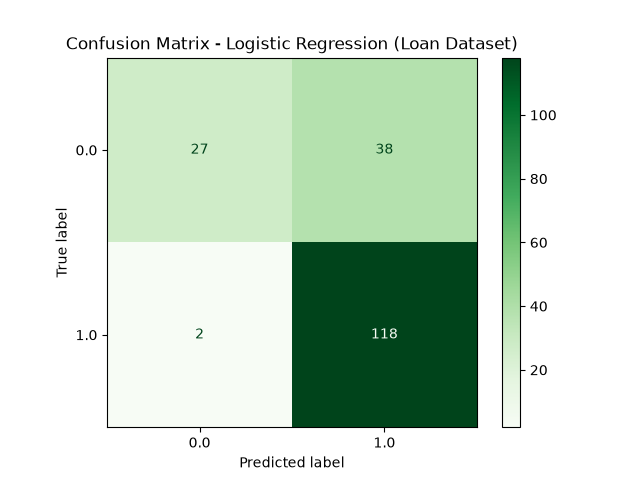
\includegraphics[width=\textwidth]{gambar/cm_loan_lr.png}
            \caption{CM Logistic Regression}
        \end{minipage}\hfill
        \begin{minipage}{0.45\textwidth}
            \centering
            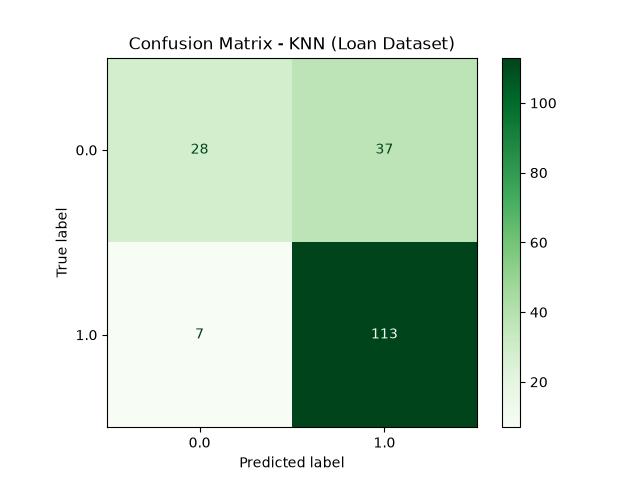
\includegraphics[width=\textwidth]{gambar/cm_loan_knn.png}
            \caption{CM KNN}
        \end{minipage}
        
        \vspace{0.5cm}
        \begin{minipage}{0.45\textwidth}
            \centering
            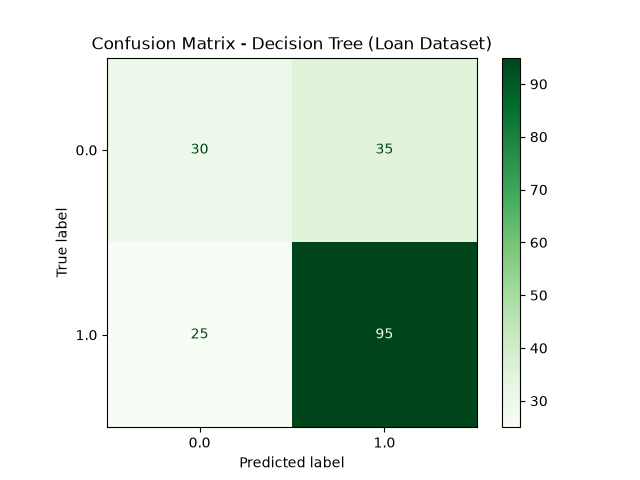
\includegraphics[width=\textwidth]{gambar/cm_loan_dt.png}
            \caption{CM Decision Tree}
        \end{minipage}\hfill
        \begin{minipage}{0.45\textwidth}
            \centering
            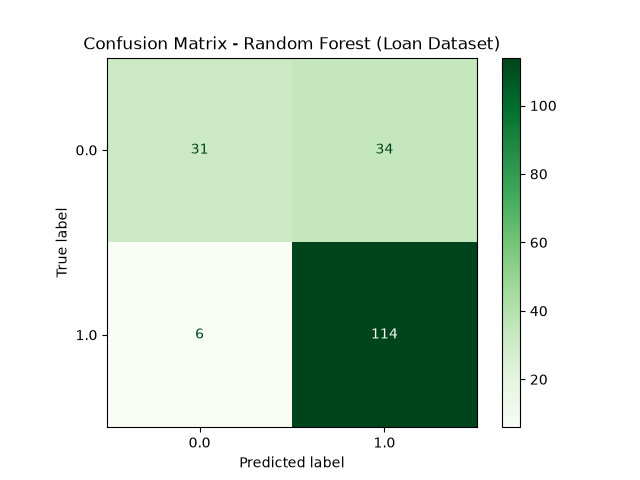
\includegraphics[width=\textwidth]{gambar/cm_loan_rf.png}
            \caption{CM Random Forest}
        \end{minipage}
    \end{figure}

    \item \textbf{Tabel Performa Klasifikasi Pinjaman} \\
    Dari hasil komputasi prediksi, berikut diringkas performa skor klasifikasi.

    \begin{table}[H]
    \centering
    \caption{Perbandingan Performa Model Klasifikasi Pinjaman Bank}
    \label{tab:loan_performance}
    \vspace{0.2cm}
    \footnotesize
    \rowcolors{2}{gray!10}{white}
    \begin{tabularx}{0.8\textwidth}{X c c c}
    \toprule
    \rowcolor{darkblue}
    \thead{Model} & \thead{Accuracy} & \thead{Precision} & \thead{Recall} \\
    \midrule
    Logistic Regression & 0.7838 & 0.7564 & 0.9833 \\
    K-Nearest Neighbors & 0.7622 & 0.7533 & 0.9417 \\
    Decision Tree & 0.6757 & 0.7308 & 0.7917 \\
    Random Forest & 0.7838 & 0.7703 & 0.9500 \\
    \bottomrule
    \end{tabularx}
    \end{table}

    \item \textbf{Analisis Model Terbaik} \\
    Menganalisis Tabel \ref{tab:loan_performance}, model \textbf{Random Forest} adalah model klasifikasi terbaik yang direkomendasikan. Walaupun tingkat akurasinya setara dengan Logistic Regression (sebesar 78,38\%), Random Forest mengungguli pada aspek \textit{precision} yaitu sebesar 77,03\%. Dalam konteks persetujuan pinjaman, presisi mengukur kehati-hatian model agar tidak menyetujui peminjam yang profil kreditnya bermasalah (\textit{False Positive}). Penggunaan arsitektur ansambel pohon pada Random Forest menjadikannya kuat menavigasi kompleksitas tanpa jatuh pada perangkap porsi korelasi yang mendominasi, sehingga evaluasi profil pinjaman lebih objektif dan aman bagi instansi perbankan.

\end{enumerate}

\clearpage

%======================================================================
% BAB IV: KESIMPULAN
%======================================================================
\chapter{Kesimpulan}
Setelah melakukan eksperimen klasifikasi pada Pertemuan III, ditarik beberapa simpulan fundamental:
\begin{itemize}
    \item Algoritma klasifikasi, baik yang berbasis regresi probabilitas (Logistic Regression), pendekatan jarak spasial (KNN), pembagian keputusan (Decision Tree), hingga integrasi \textit{ensemble learning} (Random Forest dan AdaBoost) memiliki mekanisme kerja yang berbeda dalam membangun batas keputusan pembagian kelas (\textit{decision boundary}).
    \item Hasil dari dataset observasi (Stroke dan Loan) menegaskan bahwa metrik akurasi tunggal (\textit{Accuracy}) seringkali bersifat menyesatkan, terutama pada kasus \textit{imbalanced dataset}. Akurasi yang tinggi pada model Stroke didominasi oleh prediksi tebakan mayoritas absolut tanpa kemampuan memprediksi sampel kelas positif yang riil.
    \item Metrik pendamping seperti \textit{Precision} dan \textit{Recall} adalah kunci evaluasi model sejati. Khusus pada mitigasi perbankan untuk menyetujui pinjaman, \textit{precision} tinggi pada model seperti Random Forest sangat vital dalam meminimalisasi risiko penyaluran kredit gagal bayar (\textit{False Positive}).
\end{itemize}
\clearpage

%======================================================================
% DAFTAR PUSTAKA
%======================================================================
\begin{thebibliography}{99}
\addcontentsline{toc}{chapter}{Daftar Pustaka}

\bibitem{ref1}
Russell, S., \& Norvig, P. (2020). \textit{Artificial Intelligence: A Modern Approach} (4th ed.). Pearson.

\bibitem{ref4}
Han, J., Pei, J., \& Tong, H. (2022). \textit{Data Mining: Concepts and Techniques} (4th ed.). Morgan Kaufmann/Elsevier.

\bibitem{ref6}
Pedregosa, F., Varoquaux, G., Gramfort, A., Michel, V., Thirion, B., Grisel, O., Blondel, M., Prettenhofer, P., Weiss, R., Dubourg, V., Vanderplas, J., Passos, A., Cournapeau, D., Brucher, M., Perrot, M., \& Duchesnay, \'E. (2011). Scikit-learn: Machine Learning in Python. \textit{Journal of Machine Learning Research}, 12, 2825--2830.

\end{thebibliography}

\end{document}
